\chapter{Implementation Details}
\label{sec:implementation-details}



\section{SECube Firmware}
SEcube is the smallest re-configurable silicon combining three main cores in a single-chip design. Low-power ARM Cortex-M4 processor, a flexible and fast Field-Programmable-Gate-Array (FPGA), and an EAL5+ certified Security Controller (SmartCard) are embedded in an extremely compact package. This makes it a unique security environment where each function can be optimised, executed, and verified on its proper hardware device \cite{secubesite}.
The SECube device has been the selected platform that allowed to build the entire Secure Password Manager application on top of it. This is due to, as introduced before, to all the security feature that are intrinsically implemented in the chip itself, both from the point of view of the hardware and software.\newline\newline
In fact, one of the most important security enabling technology is the 3D SiP (System-in-package); the device consists of a number of integrated circuits, each one built on top of the others and enclosed into a single package.\newline\newline
Not only the system is secure from the hardware point of view, that is the necessary condition in order to develop a secure software, but the already present firmware includes some high level functions to generate a secure channel only after the authentication.

Authentication is performed from both parties, in which not only the firmware checks the authenticity of the Host but, the also the Host can do the same. This is possible thanks to a pre-shared key that is stored in the device at the very first initialization of the device itself. A custom C program, after the firmware has been uploaded, allows to setup the master password for the Secure Password Manager. This implies that the password used to authenticate the Host application is configurable only once, allowing to simplify the entire authentication process for the new feature without reducing the security. Further consideration about the user usability and the security aspects are available at Section \ref{sec:weakness}.\newline\newline
The authentication is performed using a challenge-based authentication from both sides using a MAC (Message Authentication Code) implementation called Hash-based Message Authentication Code (HMAC), that uses a secret and an hash algorithm to verify the solution of the challenge. The challenge is created thanks to the internal TRNG (True Random Noise Generator), that is an hardware included in the chip that generates a true random sequence of bits. Once the challenge has been sent to the party to be authenticated and solved, the solution is read back and checked. If it corresponds to the expected one, the party is authenticated and the channel create. A small possible weakness study is available at \ref{sec:weakness}.

\subsection{Flash memory management}
Data are saved in the internal Flash memory, by using a C structure define as follow: 
\begin{lstlisting}[style=CStyle]
	typedef struct se3_flash_pass_ {
		uint32_t id;
		uint16_t host_size;
		uint16_t user_size;
		uint16_t pass_size;
		uint8_t* host;
		uint8_t* user;
		uint8_t* pass;
	} se3_flash_pass;
\end{lstlisting}
The Image \ref{fig:sepassrecord} shows a simplified representation of all the used field.
\begin{figure}[H]
	\centering
	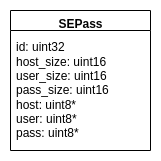
\includegraphics[width=0.2\linewidth]{images/firmware/sepass_record}
	\caption{SECube firmware password record represented using ER database schema}
	\label{fig:sepassrecord}
\end{figure}

Internally, some checks has been performed in order to inhibit the user to enter twice the same password record. This check is based on evaluating if the pair hostname and username is already present, and it is performed when the user modifies or creates a new password record. This has been made on purpose, since it has been assumed that a user can have two accounts for the same site and, even if wrong, he or she can use the same password for both of them. This has been implemented using a support method available in \texttt{se3\_pass.c} file, refer to Code \ref{code_sepass_equal}.

More precisely, data are stored in the Flash memory using as few bits as possible to make the implementation able to store a large number of passwords, accordingly to the following table:
\begin{table}[H]
	\begin{tabular}{ |c c l| }
		\hline
		\textbf{Field name} & \textbf{Number of bytes} & \textbf{Description}\\ 
		\hline
		\texttt{id} & 4 & Id to univocally identify a password, using 32 bits\\ 
		\hline
		\texttt{host\_size} & 2 & Number of characters in the \texttt{host} \\  
		\hline
		\texttt{user\_size} & 2 &  Number of characters in the \texttt{user} \\  
		\hline
		\texttt{pass\_size} & 2 &  Number of characters in the \texttt{pass} \\  
		\hline
		\texttt{host} & \texttt{host\_size} & Hostname of the password record \\  
		\hline
		\texttt{user} & \texttt{user\_size} & Username of the password record\\  
		\hline
		\texttt{pass} & \texttt{pass\_size} & Plain text of the password record\\  
		\hline
	\end{tabular}
	\caption{Flash memory for storing a Password record}
	\label{tab:flashmem_pass}
\end{table}

The adopted solution allows to use 4 bytes for the id, and 2 bytes for the hostname, username and password length. The length of the other parameters are dependent on the previous three. This implies that at maximum $2^{16} = 65536$ characters can be used for hostname, username and password, but the system is able to reduce at minimum the occupied size, since the stored bits are not fixed.\newline\newline
Data into the Flash memory are stored as defined by the C structure shown at Table \ref{tab:flashmem_pass}. Since the internal embedded Flash memory is limited, a possible attack could rely on the fact that creating few records with the hostname, username and password length set to the maximum could fill up the space. This corresponds to a DoS (Denial of Service) attack, making the system not more fully usable, by saturating the internal memory.

A solution to this problem could be to limit the number of characters of the hostname, username and password itself to a maximum value. The problem is that even in this case, if the user has an access to the device and it is logged in, he or she will be able to saturate the memory, independently from the dimension of each field. For this reason and for possible future improvements based on using the unused bits in the fields, 2 bytes have been reserved for each field.


\subsection{Code implementation}

The entire solution has been developed using the C language and everything has been built on top of the already present firmware.

Besides all the adaptations to the code that has been necessary to the Secure Password Manager to work correctly, everything is based on two C files under the ``\textit{SEcube USBStick Firmware/Project/Src/Device}" directory:
\begin{itemize}
	\item \texttt{se3\_sepass.c}
	\item \texttt{se3\_pass.c}
\end{itemize}

A coarse grain classification can be done on the level of data manipulation that the functions inside each one of the two files contains. In the case of \texttt{se3\_sepass.c}, functions are much more command oriented, allowing to perform rather complex operation by calling directly a function from the just received command. On the other hand, \texttt{se3\_pass.c} includes the functions for directly managing the Flash memory and abstract over some redundant operations, like the fetch from the storage. 


\subsubsection{Command dispatcher}
The \texttt{se3\_dispatcher\_core.c} file contains the code implementation for managing the custom commands that are necessary to provide to the Host application, in order to manage the passwords.\newline\newline
In order to add the five different commands needed to manage all the Secure Password Manager features (add, delete, modify, search and password generation), a custom command, with id 13 has been added. The five methods have been added by exploiting the sub-command management; part of the command payload is used to identify the id of the method to call. The implementation and management is available at Code \ref{code_command_disp}.

\begin{lstlisting}[style=CStyle,caption="Code for searching if password record is already present", label=code_command_disp,breaklines=true]
	uint16_t sepassword_manager_utilities(uint16_t req_size, const uint8_t* req, uint16_t* resp_size, uint8_t* resp)
	{
		uint16_t operation; // the type of operation to be executed
		memcpy((void*)&(operation), (void*)req, 2);
		se3_flash_it it = { .addr = NULL};
		if(!login_struct.y)
		{
			return SE3_ERR_ACCESS;
		}
		
		se3_flash_it_init(&it);
		it.addr = NULL;
		switch (operation)
		{
			case SE3_SEPASS_OP_ADD:
			return add_new_password(req_size, req+2, resp_size, resp);
			break;
			case SE3_SEPASS_OP_MODIFY:
			return modify_password(req_size, req+2, resp_size, resp);
			break;
			case SE3_SEPASS_OP_DELETE:
			return delete_password(req_size, req+2, resp_size, resp);
			break;
			case SE3_SEPASS_OP_GET_BY_ID:
			return get_password_by_id(req_size, req+2, resp_size, resp);
			break;
			case SE3_SEPASS_OP_GETALL:
			return get_all_passwords(req_size, req+2, resp_size, resp);
			break;
			case SE3_SEPASS_OP_GENERATE_RANDOM:
			return generate_random_password(req_size, req+2, resp_size, resp);
			break;
			default:
			SE3_TRACE(("[sepassword_utilities] invalid operation\n"));
			return SE3_ERR_PARAMS;
		}
		return SE3_OK;
	}	
\end{lstlisting}



\subsubsection{se3\_pass.c}
As already introduced before, the \texttt{se3\_pass.c} contains all the low level operations with the Flash memory. The most important available methods are the following:
\begin{itemize}
	\item \texttt{se3\_pass\_find}: given a password id, returns true if that id used
	\item \texttt{se3\_pass\_new}: given a password record, creates a new password record in the Flash memory
	\item \texttt{se3\_pass\_read}: reads from the Flash memory the password information of a single password
	\item \texttt{se3\_pass\_equal}: returns true if there is a password with the same hostname and same username. The implementation is available at \ref{code_sepass_equal}
\end{itemize}

\begin{lstlisting}[style=CStyle,caption="Code for searching if password record is already present", label=code_sepass_equal,breaklines=true]
	bool se3_pass_equal(se3_flash_pass* password, se3_flash_it* it)
	{
		bool areEquals = false;
		se3_flash_pass tmp;
		se3_flash_it_init(it);
		
		while (se3_flash_it_next(it) && !areEquals)
		{
			if (it->type == SE3_TYPE_PASS)
			{
				se3_pass_read(it, &tmp);
				
				if (tmp.id == password->id || (is_str_eq(tmp.host, tmp.host_size, password->host, password->host_size) && is_str_eq(tmp.user, tmp.user_size, password->user, password->user_size)))
				{
					areEquals = true;
				}
				
				if(tmp.host != NULL) {free(tmp.host);}
				if(tmp.user != NULL) {free(tmp.user);}
				if(tmp.pass != NULL) {free(tmp.pass);}
			}
		}
		
		return areEquals;
	}
\end{lstlisting}



\subsubsection{se3\_sepass.c}
\label{sec:se3_sepass.c}
Differently form the \texttt{se3\_pass.c} file, the \texttt{se3\_sepass.c} contains high level oriented functions that are directly called by the sub-command command dispatcher for the password manager.\newline\newline
The available methods are the following:
\begin{itemize}
	\item \texttt{add\_new\_password}: used to generate a new password. The parameters such as the hostname, the username and the password are extracted from the command parameters and checked against the current state of the Flash. More precisely, besides the consistency checks that are performed before parsing the parameters, the pair hostname and username is searched into the memory, if not present the new password record is created. One important aspect is that the id of the new password is generated outside the device, and it is duty of the Host application to provide a valid value. This has been done in order to increase the flexibility of the solution and to allow the Host to use any kind on enumeration.
	\item \texttt{modify\_password}: similarly form the \texttt{add\_new\_password} function, the parameters are read and checked. Only if the id is present, the previous record is deleted and replaced by the new one with all the correct information.
	\item \texttt{delete\_password}: this simply deletes the password record by a given id
	\item \texttt{get\_all\_passwords}: returns a list of all the passwords. It is also possible to filter by username or hostname
	\item \texttt{get\_password\_by\_id}: given an id, the password record is returned
	\item \texttt{generate\_random\_password}: given the length and the set of characters that must be used, a random password is generated using the internal TRNG.
\end{itemize}

The password can be generated by using a combination of four different character sets:
\begin{itemize}
	\item Lowercase: abcdefghijklmnopqrstuvwxyz
	\item Uppercase: ABCDEFGHIJKLMNOPQRSTUVWXYZ
	\item Number: 1234567890
	\item Symbol: -\_.:;,?\&\%\$!\@\#
\end{itemize}

The \texttt{generate\_random\_password} method has been implemented by exploiting the TRNG that generates the number of characters in bytes. This means that if the password to be generated is 100 characters long, the TRNG will be exploited to gather 100 random bytes. 

This has been done for a specific reason, each byte is used to select a character from the set that has been generated from the union of all enabled sets.\newline\newline
This solution allows to have that each character in the cumulative set has the same probability to be used.

This solution has been choose to avoid the problem of a non-uniform distribution of each character probability. If all sets are enabled and merged together to form a single set, as in this implementation, the probability that taking a random character from the newly generated password is exactly the `\texttt{A}' one is:
\begin{center}
	Pr(X = A) = $100 \cdot \frac{1}{26+26+10+13} = 1.3 \%$
\end{center}

The firmware function used to generate a random password is based on randomly select $N$ characters from the enabled sets (alphabet lowercase and uppercase, numbers and symbols). The current implementation, is totally random but is able to ensure that at least one character from all the enabled sets is selected. This has been implemented by performing a loop over the just generated password, if it does not contains at least one character for each enabled set, the computation is repeated. In order to avoid an infinite loop, the upper limit of the number of iterations has been set to 100.


\subsection{Possible weakness}
\label{sec:weakness}
At the current state-of-the art of the implementation, there is not a way to retrieve or change the password if the used does not know the current one. This is an intrinsic weakness of the solution, since having only one factor authentication that is not supported by a second authentication method, the only way to gain access to the stored password would have been to create a support method that would have reduced the security. This generates a problem: giving the possibility to the user to retrieve the master password in some way, would have reduced the overall security. For this reason, even if the user usability could be reduced, the main focus was to not disclose the password to who is not able to be authenticated.\newline\newline
From the point of view of the HMAC used to perform the Host and Device mutual authentication the security is intrinsically provided by the fact that the secret is stored in a secure hardware. The fact that also the Host application has the ability to verify the Device using the same challenge-based authentication explained before, implies that the solution generated by the firmware has been generated by using the same shared key that is used to authenticate the Host application. The following sentences explain how an bruteforce attack could be used against this type of authentication, with focus on a particular use case.

From the Chrome Extension usability definition, the user has to enter the password in order to unlock the extension itself and be allowed to manage the password. If an attacker is doing \textit{piggyback}, he or she will see only the number of inserted character (since characters will be replaces with black dots) or some pressed keys. The problem with this is that, if the firmware solved challenge has been generated and available to the attacker in some way (like stealing the SECube for some minutes), he or she can perform a bruteforce attack. The time will be drastically reduced if come characters are known. One solution to solve this would be to not allow the Host application to authenticate the SECube itself, but this is not secure for obvious reasons. 
During the early development of this project, it was proposed to implement a delayed authentication; if the user performs $X$ wrong login attempts, the next one must be done after $Y$ seconds, otherwise an error is always generated. The fact that challenge is independently generated from the login API, makes also this solution unfeasible. The feasibility of the attack strictly depends on the importance of the stored passwords and it is a matter of effort/cost, since the high security level of the challenge used.



\section{Host Middleware}

The Host Middleware is a software intended to run in the user's PC (for example as a daemon on Linux or as a service on Windows) and to provide a secure connection between the user's PC and the SECube board. This means that it acts as a bridge between the Chromium Extension (the frontend for the user) and the board, thus the Middleware is developed with security in mind.\\

It's main job is to serve some HTTPs requests. In fact, it provides REST APIs to allow the Chromium Extension to interact with the features exposed by the SECube's firmware. This means that it acts as a web server with HTTPs support in order to provide a secure connections.

\subsection{The web server}
HTTPs is a secure protocol that uses a TLS connection to provide a secure connection between two endpoints, and it's a replacement for the HTTP protocol. This means that HTTPs provides the following benefits:

\begin{itemize}
    \item Authentication
    \item Confidentiality: the connection is encrypted and the data is encrypted
    \item Integrity: the data is signed and the signature is verified
\end{itemize}

Thus, HTTPs helps to avoid the risk of eavesdropping, which is a risk that can be exploited by an attacker to intercept the data and modify it. More in general, it avoids \textit{Man In The Middle} attacks. 

The middleware is developed mainly in Python. To implement the web server, Flask is used as module. It natively supports HTTPs and a self-signed certificate is used, generated with \textit{openssl}.\\

\subsection{The REST APIs}
The exposed APIs are totally complaint to the REST principles. It uses cookies to authenticate the user, and JSON as exchange data format. \\

The main API is the one the allows to create a session. Once a session is created (via a successful authentication), a cookie is generated and sent to the browser. The browser will then store securely the cookie and the extension will automatically attach it to each request. In the end, the cookie is strictly needed to interact with all other APIs.\\

The endpoint to create a session is \texttt{POST /api/v0/device/0/session?pin=<pin>\&enditme=<endt>}. The \texttt{pin} parameter is the PIN code of the board, used to unlock it, while the \texttt{endtime} parameter is the time in seconds until the session expires. When the session expires, the middleware will automatically invalidate it and each subsequent request will result in \texttt{403 Unauthorized}. The \texttt{endtime} parameter is a timestamp in seconds, and it's relative to the middleware's one. The middleware is capable of generating it internally and the current timestamp can be obtained via \texttt{GET /api/v0/time}. For a more complete description of the API, see the appendix \ref{api}.

\subsection{CORS Support}
One of the main issues is the enable of the Cross Origin Requests support from all the origins and to allow the session cookie to be used from any website (flag same-site set to False). The cookie alone is not a problem because the ID is a valid data only if used by the Middleware, so there is no leakage outside. \bigskip

Both the Cookie and the CORS support (so APIs are allowed to be used from external web sites with a hostname different from 127.0.0.1) expose the Middleware to some attacks (like Cross-Site Forge Requests) even if the browser should theoretically block all requests from external web sites to the localhost. CORS is required because of some APIs that will be used to enable password auto-completition, thus the request will be done by the Extension by means of the website the user is browsing in, doing a kind of code injection in the web site itself (a secure code injection because the browser allows it and the user thrust the Secure Password Manager extension). \bigskip

To achieve both auto-completition support (with CORS enabled) and high level of security from this point of view, the middleware is developed adding a filter to the requests that are done: the filter is based on the HTTP origin header. \bigskip

When a request arrives, the Middleware checks the origin field in the HTTP header: if it is not present or it is chrome-extension://* it means that the request is coming from the chromium extension so there will be no filter applied, otherwise it will contain a valid hostname and a filter is applied. The filter consists in obtaining the hostname (without protocol and other stuff, i.e. https://www.example.com will be example.com), in this way the only endpoint that will be enabled is \texttt{/api/v0/device/0/passwords?hostname=example.com}. If the required endpoint is different in any aspects from the enabled one, 403 Unauthorized will be returned otherwise the request will be processed. This means that a web site is able to access only to the passwords of that web site: it is user's responsibilities to not access and give passwords to fake web sites or to install fake chromium extensions that may access the middleware. \bigskip

This operation is completely safe because of the inhibition of the browser is any try of modifying the origin field in the HTTP header. Thus, a malicious website can't in any way modifying the origin field, allowing the middleware to block any APIs usage. An external tool can obviously write what it wants in the header (indeed can try to forge a request towards the middleware with origin: https://example.com). In that case, the middleware will block the request because the external tool doesn't contain the user's cookie so no session will be associated to this request.

\subsection{Session Management}
When a cookie is created, it contains only the session ID. This ID is used to identify the session, and it's used to identify the user. The session ID is generated by the middleware and it's unique for each session. This means that on the user's side, only the ID is stored instead of any other sensitive information. The user is protected by \textit{client identity steal} attacks thanks to the security given by the browser in storing it locally.

On the middleware side, a session corresponds to a file stored in the file system, in the same directory as the middleware's executable. The file name is the session ID. The file contains the following information:

\begin{itemize}
    \item The board's PIN given by the user when the session was created
    \item The endtime of the session (timestamp in seconds)
\end{itemize}

In order to avoid possible attacks because of the files stored in clear in the file system, the session is encrypted with a key that is generated by the middleware. At each startup of the middleware, a 2048 bit RSA key is generated and stored in the RAM, and each previously created session is invalidated and destroyed. The public/private keys are used to encrypt/decrypt on the fly the requested session file. The encryption/decryption is done on-the-fly and then the session is stored in the file system, so a non encrypted version of the file will never appear in the file system. Both the PIN and the endtime are encrypted, along with other side information.

\subsection{Timestamp and Timeout Management}
In order to avoid the risk of \textit{time-leap} or \textit{time travel} attacks, the middleware uses an internal timestamp instead of the PC's one. So, even if a malicious user changes the PC's time, the middleware's timestamp will continue to update itself correctly and sessions will expire correctly.\\

In order to generate the timestamp, the middleware uses a dedicated thread that periodically (each seconds) updates the timestamp. The same information can be accessed via \texttt{GET /api/v0/time}. The timestamp is updated each second, so it's not possible to get a timestamp that is in the past.\\

At each request, the middleware:

\begin{enumerate}
    \item finds the session file corresponding to the session ID in the request (associated to the cookie sent by the Extension)
    \item decrypts the file
    \item gets the stored endtime timestamp
    \item gets the current timestamp (so the middleware's timestamp)
    \item compares the endtime with the current timestamp and if the endtime is reached (greater or equal), the session is invalidated and the request is replied with \texttt{403 Unauthorized}
    \item gets the stored PIN
    \item tries to authenticate the user with the PIN
    \item if the \textit{login} is unsuccessful, the request is replied with \texttt{403 Unauthorized}, otherwise the request continues with the operation requested by the user 
\end{enumerate}

\subsection{How to interface Python with C++?}
As mentioned above, the middleware is developed in Python. However, the HOST libraries used to communicate with the board are written in C++. This means that the Python code needs to be able to interface with the C++ libraries. In order to do that, the middleware use the \textit{Ctypes} module. It's a builtin module that allows to interface with C libraries.\\

The actual implementation sees some wrappers (both for the \textit{L0} and \textit{L1} libraries). Those wrappers are C functions that uses only C's primitive types as arguments and as return values, because of the way ctypes works. An example of function wrapper is the following one, used to initialize the \textit{L0} library:

\begin{lstlisting}[style=CStyle]
#ifdef _WIN32
#include <Windows.h>
#define __MODIFIER __declspec(dllexport)
#else
#define __MODIFIER 
#endif

#define EXPORT_FUNC(_type, _name) extern "C" __MODIFIER _type _name

EXPORT_FUNC(void *, createL0Instance)() {
    return new(std::nothrow) L0;
}

\end{lstlisting}

Once C wrappers are all defined and implemented, all the code needs to be compiled. In this case there is no \textit{main} function, so there is no an executable file to run. Because those functions are meant to be called from the external (i.e. the Python code), the code is compiled as a shared library. On Linux, they are compiled as \textit{.so} files. On Windows, they are compiled as \textit{.dll} files. The shared library is then loaded by the Python code.\\

With ctypes, the function wrapper is easily invoked. The first thing that is done is to tell to ctypes what are the arguments and return types of the function, then the function can be called. Because this procedure must be done for each function, a python class has been created to encapsulate the functions. There is a class both for the \textit{L0} and \textit{L1} libraries, and this is an example:

\begin{lstlisting}[style=PyStyle]
class L0:
    def __init__(self, path_lib: str):
        self._libname = path_lib
        self._c_lib = ctypes.CDLL(self._libname)

        # Create L0 instance
        self._c_lib.createL0Instance.argtypes = []
        self._c_lib.createL0Instance.restype = ctypes.c_void_p

        self._l0inst = self._c_lib.createL0Instance()
\end{lstlisting}

\subsection{How to secure Python code?}
The python code is not secure. While the C code is compiled into executable code and it's a very difficult job to reverse engineer, the Python code is directly interpreted on the fly, so there is no compilation and the code is in clear. Moreover, it can suffer from \textit{code injection} attacks, so the code must be protected against those attacks.\\

In order to achieve this, a python library is used, called \textit{pyarmor}. Its first job is to obfuscate the code, so write the code in such a way it can't be understood easily by an human. This protects against \textit{code injection} and reverse engineering. The resulting obfuscated script is something like this:

\begin{lstlisting}[style=PyStyle]
from pytransform import pyarmor_runtime
pyarmor_runtime()
__pyarmor__(__name__, __file__, b'\x06\x0f...')
\end{lstlisting}

Moreover, the original python code (that now is obfuscated) is wrapped with functions that insert timers to prevent debugging and to prevent old stack traces dump. This is done by letting the python code run normally and at the end of each function call (where each function call creates a new stack frame), the frame is cleared. \\

Finally, the last precaution is to wrap everything into a single executable. The middleware is mainly composed of different python files, the shared library and the private and public keys. Using a library called \textit{pyinstaller}, the middleware is packed into a single executable. What \textit{pyinstaller} does is to create an executable that when is executed it creates a temporary folder and extract from itself all the files together with a standalone version of the python interpreter. This is done so that the middleware can be executed without the need to install the python interpreter and without the library installed. Moreover, it protects by possible \textit{code injection} attacks done at the interpreter level. The final job of pyinstaller is to encrypt the content of the executable. Because the executable needs to know the key to decrypt it when it's requested by the user, the key is hardcoded into the executable itself, so it's relatively easy to obtain the key but a malicious user needs to do some reverse engineering of the executable itself so it's an increase of time spent on trying to attack the middleware. 

% This is where you explain what you have implemented and how you have implemented it. Place here all the details that you consider important, organize the chapter in sections and subsections to explain the development and your workflow.\\Given the self-explicative title of the chapter, readers usually skip it. This is ok, because this entire chapter is simply meant to describe the details of your work so that people that are very interested (such as people who have to evaluate your work or people who have to build something more complex starting from what you did) can fully understand what you developed or implemented.\\Don't worry about placing too many details in this chapter, the only essential thing is that you keep everything tidy, without mixing too much information (so make use of sections, subsections, lists, etc.). As usual, pictures are helpful.

\section{Chrome extension}
\subsection{Tools used for the Chrome extension}

Extensions are made of different, but cohesive, components. Components can include background scripts, content scripts, an options page, UI elements and various logic files. Extension components are created with web development technologies: HTML, CSS, and JavaScript. An extension's components will depend on its functionality and may not require every option.

In this project the extension was build with the following tools:

\begin{itemize}
    \item HTML \cite{html}
    \item CSS \cite{css}
    \item Typescript \cite{ts}
    \item Node \cite{node}
    \item React \cite{react}
    \item Webpack \cite{webpack}
    \item Material-UI \cite{mui}
\end{itemize}

Let's see in the details each of these tools.

\subsubsection {HTML}

As said in the previous section, the extension is made with the web development technologies. HTML, HyperText Markup Language, is one of them.
In this project, HTML does not have a central role, since it is managed automatically by webpack. However, when the extension is build, the popup and the options main page are in HTML.

\subsubsection {CSS}

CSS, Cascading Style Sheets, is another web development technology. In this project, CSS is lightly used to style the extension's UI. The majority of the styling part is done through React and Material-UI. However, it's important to mention CSS, since it heavily used and is a key part of the web development workflow.

\subsubsection {TypeScript}

Typescript is a web development technology that is used to write code in a more readable and easy to understand way. In this project, Typescript is used to write the extension's logic.
Typescript is a syntactic superset of Javascript and adds optional static typing to the language. Another difference compared to Javascript is that Typescript is compiled and not interpreted. This means that the extension will not run unless it is compiled. The reason behind the creation of Typescript was the maintenance of large-scale applications. So the decision of using Typescript was made to make the extension's code more maintainable.
In addition, since Typescript has a static typing system, that enables static language analysis, which simplifies the development process by providing meaningful errors.
\subsubsection {Node}

Node.js is an open-source, cross-platform, back-end JavaScript runtime environment that runs on the V8 engine and executes JavaScript code outside a web browser
Node.js has an event-driven architecture capable of asynchronous I/O. These design choices aim to optimize throughput and scalability in web applications with many input/output operations, as well as for real-time Web applications (e.g., real-time communication programs and browser games).
Node.js allows the creation of Web servers and networking tools using JavaScript and a collection of "modules" that handle various core functionalities.

npm is the pre-installed package manager for the Node.js server platform. It installs Node.js programs from the npm registry, organizing the installation and management of third-party Node.js programs. Packages in the npm registry can range from simple helper libraries to task runners.

\subsubsection {React}

React (also known as React.js or ReactJS) is a free and open-source front-end JavaScript library for building user interfaces based on UI components. It is maintained by Meta (formerly Facebook) and a community of individual developers and companies. React can be used as a base in the development of single-page, mobile, or server-rendered applications with frameworks like Next.js. However, React is only concerned with state management and rendering that state to the DOM, so creating React applications usually requires the use of additional libraries for routing, as well as certain client-side functionality.

\subsubsection {Webpack}

Webpack is a free and open-source module bundler for JavaScript. It is made primarily for JavaScript, but it can transform front-end assets such as HTML, CSS, and images if the corresponding loaders are included. Webpack takes modules with dependencies and generates static assets representing those modules.
To improve security, a package called Webpack Obfuscator (\url{https://www.npmjs.com/package/webpack-obfuscator})is used to obfuscate the code. This package avoids any kind of reverse engineering of the code.
% insert image
\begin{figure}[h!]
    \vspace{0.5cm}
    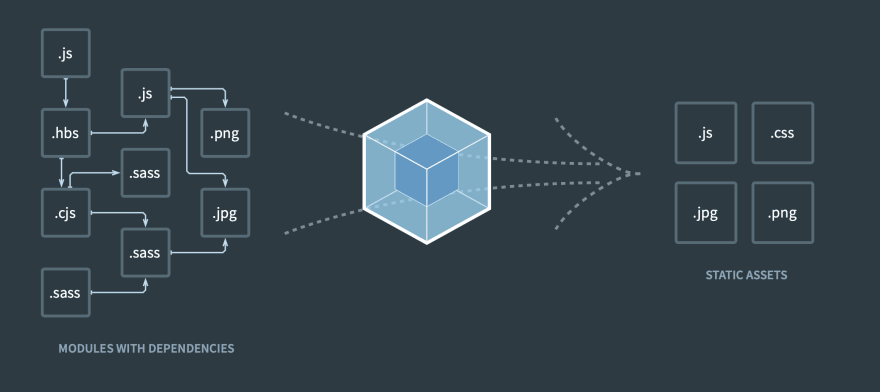
\includegraphics[width=\textwidth]{images/extension/webpack-bundle.png}
    \caption{webpack workflow}
    \label{fig:webpack-bundle} % this is the image label, with which you can refer to the image in any document location.
\end{figure}

\subsubsection {Material-UI}

Material UI is an open-source React component library that implements Google's Material Design. In this project is used to create the extension's UI.
It includes a comprehensive collection of prebuilt components that are ready for use in production right out of the box.
Material UI is beautiful by design, and features a suite of customization options that make it easy to implement your own custom design system on top of our components.
The main advantages of material UI are:

\begin{itemize}
    \item Ready to use
    \item Follow Google's Material Design so it is consistent with a big part of the web
    \item Reliable with a great community
\end{itemize}


\subsection {Design Choices}

In this section all design choices are explained. For each key part of the extension there is an image showing it and there is a complete explanation.

\subsubsection{Login}

The first page of the extension is the login page. Here there is a simple text field, in which you can enter your master password. In addition to that there is a button, to trigger the login action. If the password is correct the extension will show the main page.
The login page is shown in \autoref{fig:login}.

When clicking the login, if nothing happens, the reason is because the certificate is not trusted. In fact, on the bottom of the extension there is a text, giving brief instruction to trust the certificate. 
For a better understanding of the process of trusting the certificate, everything is explained is \autoref{sec:accept_certificate}.
This process is necessary only in the testing process, because in a real world usage, the certificate will be issued by a trusted Certificate Authority.


% insert image
\begin{figure}[h!]
    \centering
    \vspace{0.5cm}
    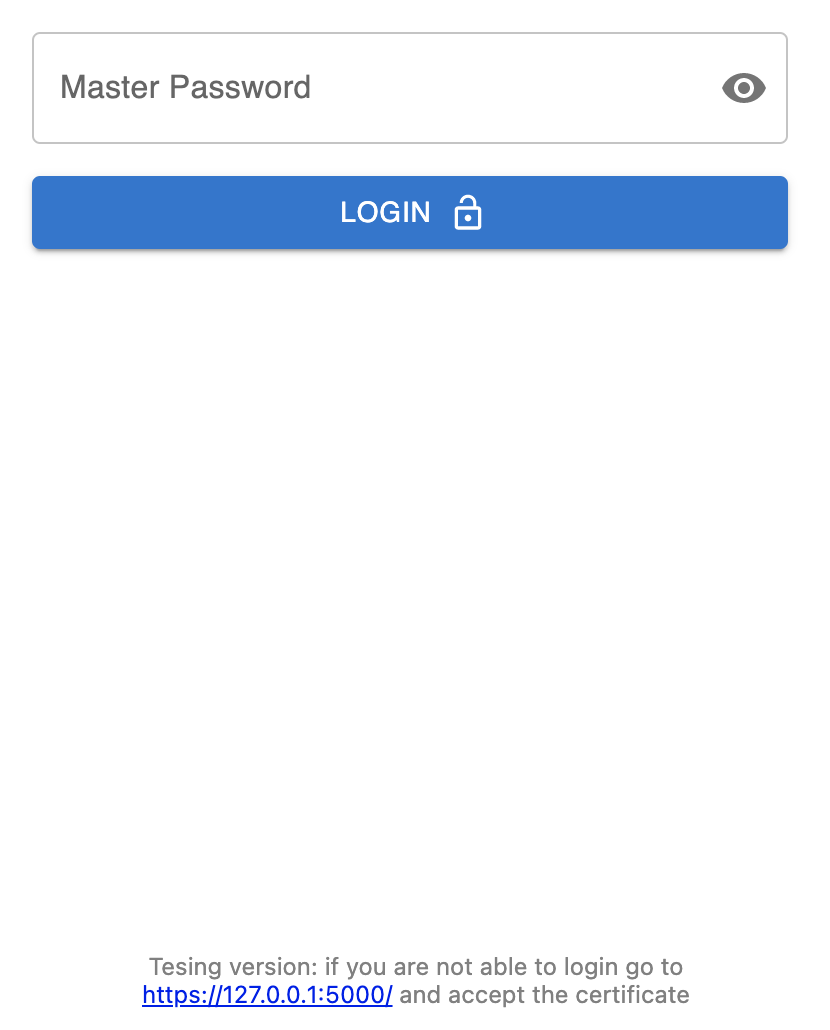
\includegraphics[width=0.4\textwidth]{images/extension/login.png}
    \caption{Login page}
    \label{fig:login} % this is the image label, with which you can refer to the image in any document location.
\end{figure}


\subsubsection {Popup and Tab Navigation}

The two key elements of the extension are the popup and the tab navigation. The popup is the main window of the extension and the tab navigation is the bottom part of the popup, in which there are the tabs that are used to navigate between the different sections of the extension. The four tabs are:

\begin{enumerate}
    \item \textbf{Tab}: it shows passwords, if there are, for the current website.
    \item \textbf{My Vault}: it shows the passwords that are stored in the vault.
    \item \textbf{Generate}: it allows the user to generate a new password.
    \item \textbf{Add}: it allows the user to add a new password.
\end{enumerate}

% insert image

Another detail in the popup is the lock button. This button, when clicked, blocks the extension. This allows the user to force lock the extension, since the next time it will be opened it will ask for the master password.
The whole popup with the component just described is shown in image \ref*{fig:popup-lock-tab}
% Insert image

% insert image
\begin{figure}[h!]
    \centering
    \vspace{0.5cm}
    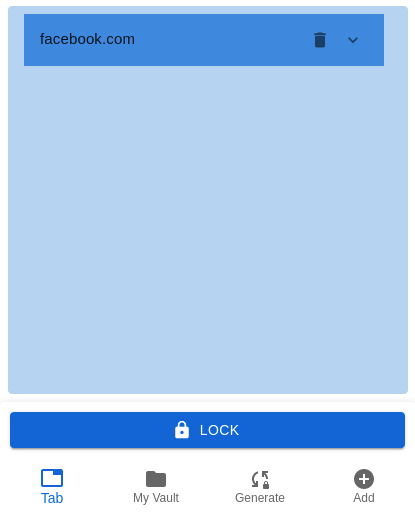
\includegraphics[width=0.4\textwidth]{images/extension/popup-lock-tab.png}
    \caption{Popup, lock button and tabs}
    \label{fig:popup-lock-tab} % this is the image label, with which you can refer to the image in any document location.
\end{figure}

\subsubsection {Tab}

The tab section of the extension is shown in image \ref{fig:popup-lock-tab}. It's visible that when the user clicks on the extension, the popup opens and the Tab is the default section. In fact, in this section, the user can see the passwords that are stored for the current website.

This is done by retrieving the hostname of the website, and then searching for the website in the vault. If the website is found, the passwords are shown.

\subsubsection {My Vault}

The My Vault section is shown in image \ref{fig:my-vault}. It's visible that when the user clicks on the extension, the popup opens and the My Vault is the default section. In fact, in this section, the user can see the passwords that are stored in the vault.
% insert image
\begin{figure}[h!]
    \centering
    \vspace{0.5cm}
    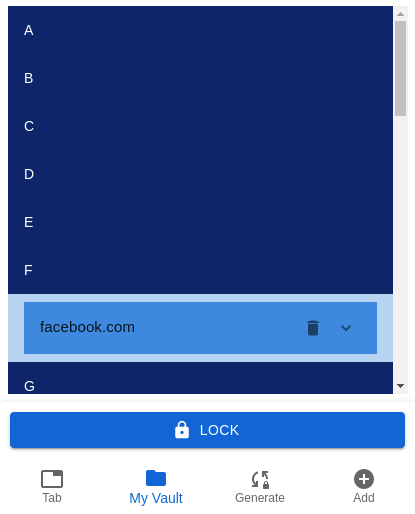
\includegraphics[width=0.4\textwidth]{images/extension/my-vault.png}
    \caption{My Vault section of the extension}
    \label{fig:my-vault} % this is the image label, with which you can refer to the image in any document location.
\end{figure}

\subsubsection{Generate}

% insert image
\begin{figure}[h!]
    \centering
    \vspace{0.5cm}
    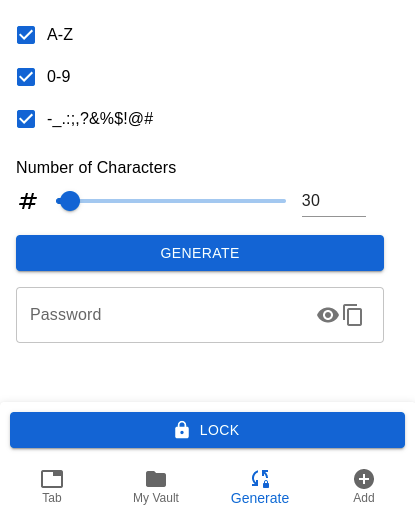
\includegraphics[width=0.4\textwidth]{images/extension/generate.png}
    \caption{Generate section of the extension}
    \label{fig:generate} % this is the image label, with which you can refer to the image in any document location.
\end{figure}

This section is very important, since it is used to generate a new password. The user can choose the length of the password, and the type of characters that will be used. The supported type of characters are:

\begin{itemize}
    \item \textbf{Uppercase}: uppercase letters
    \item \textbf{Numbers}: numbers
    \item \textbf{Special}: special characters
\end{itemize}
If no type of characters is selected, the password will be generated with lowercase letters only.
The generated password is shown in image \ref{fig:generate}

\subsubsection{Add}

The last section of the extension is the Add, that is useful to add a new password to the vault. The logic behind the autocompletion of the hostname is the same as the one from the Tab section.
The Add section is shown in image \ref{fig:add}

% insert image
\begin{figure}[h!]
    \centering
    \vspace{0.5cm}
    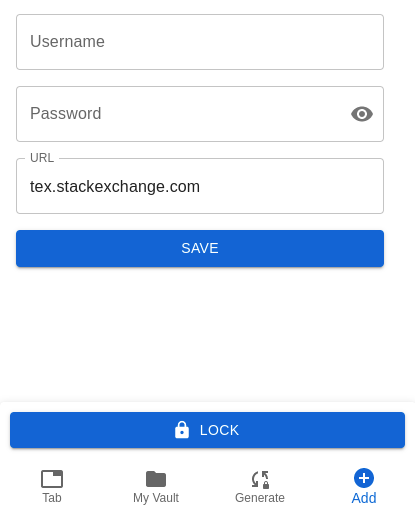
\includegraphics[width=0.4\textwidth]{images/extension/add.png}
    \caption{Add section of the extension}
    \label{fig:add} % this is the image label, with which you can refer to the image in any document location.
\end{figure}


\subsection{Options}

The options are kept as simple as possible. In fact there are only two of them:

\begin{enumerate}
    \item \textbf{Autocomplete}:it allows to autocomplete the login form when the page is uploaded
    \item \textbf{Lock After}: it allows to specify the minutes after which the extension will be locked and ask again the password.
\end{enumerate}

In order to retrieve the options when the users reopens the extension, the local storage is used. Since the options are not sensible data, it is not important that the data are encrypted, and in fact the local storage was the correct choice. In a future implementation, since Chome support by default the sync storage, the options can be stored in the sync storage so that each Chrome browser connected to the same Google account will have the same options. This uses the Google sync API and it can be taken as it is, supposing it is secure out of the box. 

% insert image

\subsection{Expandable Menu and Buttons}

In the section of the extension where we have the entries with the password, there always is a expandable menu. When expanded, the entry shows the username, the password and the URL. 

To improve security, the password is hidden by default. This rule applies to all field where there is a password. However, if the user wants to see the password, there is an eye button at the end of the password field, that allows to show the password.

When the menu is expanded, near each field there are two buttons:

\begin{enumerate}
    \item \textbf{Edit}: it allows to edit the field
    \item \textbf{Copy}: it copies the content of the field to the clipboard.
\end{enumerate}

In addition to the expandable menu there is also a button that allows to delete the password. When the button is clicked, the user is prompted with a confirmation dialog. The button of the confirmation dialog are colored in a way such that the delete button is red, and the keep button is green.


\subsection{Autocomplete}

This feature is a key part of the extension, since it improves drastically the user experience and usability. The extension is able to autocomplete the login form when the page is loaded. 
The idea behind the autocomplete is the following: when the page is loaded, the extension retrieves the username and password text fields. Then, the extension, knowing the current website, makes a request to the Middleware to retrieve the username and password of the website. If the username and password are found, the extension automatically fills the fields. Otherwise, nothing happens.

The autocomplete feature works in conjunction with the lock after. In fact, if the extension is locked, the autocomplete feature is disabled. Indeed, if the extension is unlocked, the autocomplete feature follows what the user set in the options.
\subsection{Lock After}

This feature is very important from two points of view: first, it allows the user to keep the extension unlocked for a certain period of time avoiding the need to enter the password every time the extension is opened. Second, it allows the user to lock the extension after a certain period of time, and ask again the password. So it touches both usability and security, finding a balance between the two. The balance stands is the customizability; in fact the time, in minutes, after which the extension will be locked is configurable in the options. 

The implementation is pretty straightforward. When the user unlocks the extension, a timestamp is sent to the Middleware, that saves it. After that, at every request, the Middleware checks if the current timestamp is greater than the saved timestamp. If it is, the Middleware returns 403, and so the extension is locked. Otherwise, the Middleware returns the asked data. 
